\documentclass[a4paper]{article}
%Commented in draft to allow for notes.
\usepackage{fullpage}
\usepackage{hyperref}
\usepackage{todonotes}

\title{Robotic Swarms: \\Distributed Coordination Without Location}
\author{S.J.A. Bekhoven  \and
    S.P. Metman \and
    M.J. Rogalla}
\date{\today}

\pagestyle{empty}

\begin{document}
\maketitle
\thispagestyle{empty}

\begin{abstract}
This is the abstract of my paper.
This is the abstract of my paper.
This is the abstract of my paper.
This is the abstract of my paper.
This is the abstract of my paper.
This is the abstract of my paper.
This is the abstract of my paper.
This is the abstract of my paper.
This is the abstract of my paper.
This is the abstract of my paper.
This is the abstract of my paper.
This is the abstract of my paper.
\end{abstract}

% Do not compile individual files, compile only this main file.

\section{Introduction}
  %!TEX root = ../Bachelorseminar-RoboticSwarms.tex

Swarm robotics has become a prominent and promising research area in the recent years. 
It has great potential use for a large variety of applications, some of which have already been successfully implemented. 
We want to provide a global overview of the main problems found in the research area of robotic swarms. 
Many articles already exist which give an overview of applications and used practices in this area, but often do not explain the problems underlying these practices. 
Therefore, we focus on providing a problem-oriented overview of the robotic swarms, while also providing a general overview of best practices and solutions of these problems.\\
\\
We start by defining some terminology, since some of the terms used in robotic swarms are ambiguous and can be interpreted in different ways.
We define a swarm as a scalable network of robots which consists out of more than two robots.
Furthermore, we only consider robotic swarms in which every robot has some form of distributed intelligence.
An exception is of course when a swarm of multiple robots is controlled by one control station.
Because the swarm robots have to communicate either directly or indirectly with each other, the swarm will still have some form of distributed intelligence to function.
% Thus, according to our original definition, we still regard it as a swarm. \\
\\
\\
Robotic swarm algorithms can roughly be characterized by their location type and their information type. Algorithms can then respectively be either \emph{location-based} or \emph{location-free} and either \emph{range-based} or \emph{range-free}:
\begin{description}
	\item[Location-free] Robots have no knowledge and do not keep track of their absolute or relative location.
	%A robotic swarm is \emph{location-free} if the swarm has no knowledge of the boundaries of the location it is in, whether it is provided at the beginning or is actively searched for during the execution of the algorithm. 
	\item[Location-based] Robots have perfect knowledge or keep track of their absolute or relative location.
	%A robotic swarm is \emph{location-based} if each individual robot in the swarm has the knowledge of its absolute or relative location.
	\item[Range-free] Robots do not communicate or communicate via some kind of central base.
	%A robotic swarm is \emph{range-free} if each robot can detect the presence of other nearby robots or obstacles, but does not store or measure the distance towards the other object.
	\item[Range-based] Robots communicate within predetermined range.
	%A robotic swarm is \emph{range-based} if each robot in the swarm keeps track of the exact distance between itself and the other robots in the swarm or obstacles. 
\end{description}

In the following sections, we compare the algorithms by two characteristics. 
The first characteristic is \emph{scalability}, by which we mean the ability of maintaining performance when the population in the robot swarm is increased. 
The second is \emph{performance}, by which we mean the general efficiency. 
We define efficiency separately for each problem before comparing the algorithms of that problem. 
We do this because the solutions have different ways of expressing efficiency for each problem.\\

A composite problem is a problem composed of multiple main problems in such a way that these main problems influence the working of the solutions. 
Although such a composite problem can be singled out, a lot of the main problems have some form of overlap too, although not with significant impact. 
The main problems Dispersion and Source Localization both include the Formation problem, and the Collective Transport is composed of the Formation problem among others.
The Exploration problem is more of an extension to the Dispersion problem. 
This relationship is shown in the Figure~\ref{fig:ProblemsOverview} \\
\begin{figure*}
  \centering
  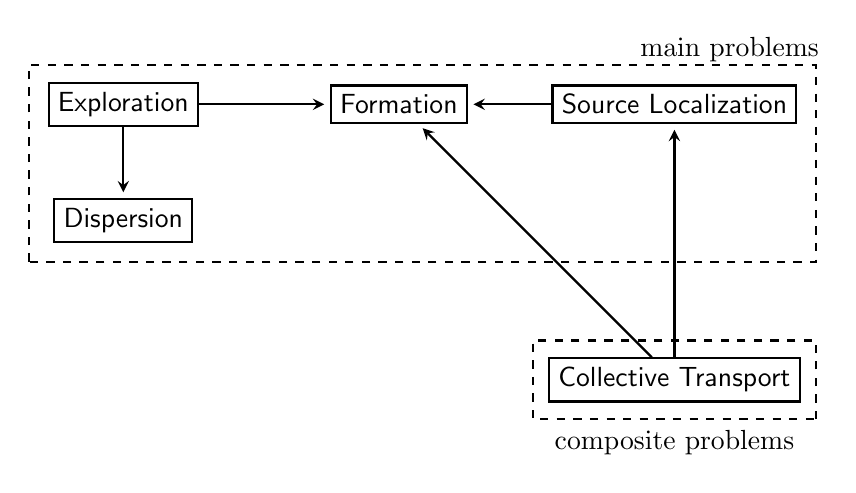
\begin{tikzpicture}[->,>=stealth,shorten >=2pt,auto,node distance=3.5cm,
    thick,main node/.style={fill=white,draw,font=\sffamily}]
    \node at (7.7,0.7) {main problems};
    \node at (7,-4.3) {composite problems};
    \draw[fill=white,dashed] (-1.2,-2) rectangle (8.8,0.5);
    \draw[fill=white,dashed] (8.8,-4) rectangle (5.2,-3);
    \node[main node] (1) {Exploration};
    \node[main node] (2) [below= 0.9cm of 1] {Dispersion};
    \node[main node] (3) [right of=1] {Formation};
    \node[main node] (4) [right of=3] {Source Localization};
    \node[main node] (5) [below of=4] {Collective Transport};

    \path[every node/.style={font=\sffamily\small}]
      (1) edge [right] node[left] {} (2)
      (4) edge [right] node[left] {} (3)
      (5) edge [right] node[left] {} (4)
      (5) edge [right] node[left] {} (3)
      (1) edge [right] node[left] {} (3);
  \end{tikzpicture}
  \caption{Problem Composition Overview} \label{fig:ProblemsOverview}
\end{figure*}



The remainder of this paper is then structured as follows. 
In Section~\ref{sec:Formation} until Section~\ref{sec:Localization} we define the main problems in robotic swarms. 
Then, in Section~\ref{sec:CollectiveTransport}, we discuss the composite problem Collective Transport. 
For each problem we mention the possible real-life applications, their subproblems and the underlying algorithms of the solutions.
After that we discuss the characteristics of each algorithm, the corresponding (dis)advantages and where possible some remaining problems.
For more information on the operation of the mentioned algorithms, you can check the references provided. 
Finally we briefly discuss our observations in Section~\ref{sec:Discussion}.




  
\section{Applications}
  %!TEX root = ../Bachelorseminar-RoboticSwarms.tex
Robotic swarms can be used for many real-world applications as for example in tasks that cover a region, tasks that are to dangerous for human beings, tasks that scale-up or scale-down in time or tasks that require redundancy \cite{csahin2005swarm}.

  \subsection{Spot Exploration}
  \textbf{Description: }\emph{Cleaning/exploring a component in an unkown area is a common problem which can be solved effectively by using a tobotic swarm. For example in \cite{wagner2008cooperative} a swarm of robots is placed in a certain component which has to be cleaned totally. The robots have limited visibility and can only see other robots within a certain distance. Main goal is to not disconnect the component that has to be cleaned to be sure that the component will be get fully cleaned in the end.} \\
  The main techniques that are described in \cite{wagner2008cooperative} are algorithms that preserve the connectivity of the spot to be cleaned and prevent the clustering of robots.
  
  \subsection{Area Exploration}
  \textbf{Description: }\emph{Exploration of an unkown environment can be done conveniently using robotic swarms. This can be very useful in cases of hazardous environments. In \cite{sheng2006distributed} a model is described in which the robots have limited communication range and full knowledge of their location. By continuously looking for the closest undiscovered area in combination with a nearness measure it tends to explore the complete area by staying together and continiously updating each others maps.} 
  
  Some of the techniques used are communication, exploration, dispersion, mapping. \cite{sheng2006distributed}
  
  \subsection{Swarm-Assisted Fire Fighting}
  \textbf{Description: }\emph{Swarm-Assisted Fire Fighting makes interactive use of autonomous robots in fire emergency settings. These swarms of robots are capable of supporting and enhancing fire fighting operations co-operatively with each other and are coordinated by a single human supervisor.}\cite{Naghsh2008,Penders2011}\\

  The techniques required for Swarm-Assisted Fire Fighting include, but are not limited to: \emph{foraging}, \emph{formation}, \emph{mapping} and \emph{exploration}.\cite{Naghsh2008,Penders2011}\todo[inline]{Check more sources and verify techniques} The foraging techniques are needed in order to give the swarm the ability to search and locate victims. Formation is required in order for the swarm to navigate optimally and prevent conflicts in exploration. The mapping and exploration service are required to create a well constructed map of the explored area, such that the human and other robots are aware of their surroundings, even if it is impossible to get a visual due to reduced visibility caused by smoke.

  \subsection{Toxic Emition Source Discovery by Robotic-Swarms}
  \textbf{Description: }\emph{Due to the ambiguity of this name, there have been many applications which have aimed to achieve this, from nuclear spills and oil spills to fire-origins. Much of this however is theoretical work, due to the fact that the price of these individual robots is still rather high.}

  Some of the techniques used in toxic source discovery are: control, communication and distribution.\cite{Li2012}
  
  \subsection{Draft}
  Give an overview of real-world applications possible with Robotic Swarms. A list of possible applications:
    \begin{enumerate}
      \item Cleaning
      \item Space Exploration (swarm of Mars rovers)
      \item Rescue Missions
      \item Treacherous Radioactive Survey
      \item Survey and cleanup of Toxic Spills
      \item Surveillance
    \end{enumerate}
  \textbf{Categories}
    \begin{itemize}
      \item Region Covering
      \item Dangers
      \item Scaling in time
      \item Redundancy
    \end{itemize}
  
  
\section{Definitions from Literature}
  \section{Definitions from Literature}

  \subsection{Orientation}
  Location-based vs Range-based \ldots
  \subsection{Applications}
  List of applications.... idea for table: Orientation Table: LB RB LF RF\\
  
  \begin{tabular}{|p{3cm}|p{3cm}|p{3cm}|}
    \hline
     & Location-based & Location-free\\\hline
    Range-based & \ldots & \\\hline
    Range-free & \ldots & \\
    \hline
  \end{tabular}
  
  \subsubsection{Service Required}
  

\section{In-depth review of Services}
  \input{./tex/5-Services.tex}

\section{Unsolved Problems}
  \input{./tex/7-UnsolvedProblems.tex}

\section{Discussion}
  %!TEX root = ../Bachelorseminar-RoboticSwarms.tex

NOTES

- scalability, global communication, 
- lots of overlap

WHAT WE MISS
- mapping
- foraging
- target localization?
- robot localization

In the past sections, we reviewed the most common problems found in the field of robotic swarms. 
These problems however, do overlap, because the problems found in this field often consist of multiple different problems. 
We focused on each problem, highlighting the communication methods of every solution and properties of these communication methods. 
These properties can be summarized in a Venn diagram, allowing for a compact overview of these solutions. 

	\begin{figure}[!ht]
		\label{venn_diagram}

		\centering

		\def\loclb{(180:2.0cm) circle (2.0cm)}
	  	\def\loclf{(0:2.0cm) circle (2.0cm)}
	  	\def\locrb{(90:2.0cm) circle (2.0cm)}
	  	\def\locrf{(270:2.0cm) circle (2.0cm)}

	    \begin{tikzpicture}
			% standard figures
			\draw \loclb node [text=black] {Location-based};
			\draw \loclf node [text=black] {Location-free};
			\draw \locrb node [text=black] {Range-based};
			\draw \locrf node [text=black] {Range-free};

			% Range-based location-free
			\draw[dashed,-] (1,1) -- (2,5.5) node[anchor=north west] {};
			\node[draw,align=left,anchor=west] at (2,5.5) {
				Leader-follower \ref{sec:Formation}\\
				Virtual structure \ref{sec:Formation}\\
				Virtual space \ref{sec:Formation}\\
				Teamwork control \ref{sec:Formation}
				Particle Swarm Optimization \ref{sec:Localization}\\
				Glowworm Swarm Optimization \ref{sec:Localization}\\
				Pheromone \ref{sec:CollectiveTransport}\\
				Heterogeneous granular convection WLC \ref{sec:CollectiveTransport}\\
				Random Walk \ref{sec:Dispersion}\\
				Follow wall \ref{sec:Dispersion}\\
				Directed Dispersion \ref{sec:Dispersion}\\
				Seek open \ref{sec:Dispersion}\\
				Fiducial \ref{sec:Dispersion}\\
				Clique-intensity \ref{sec:Dispersion}
			};

			% Range-free, location-free
			\draw[dashed,-] (1,-1) -- (2,-4.5) node[anchor=north west] {};
			\node[draw,align=left,anchor=west] at (2,-4.5) {
				Behavior-based \ref{sec:Formation}
				Fuzzy control \ref{sec:Formation}\\
				Flocking \ref{sec:CollectiveTransport}\\
				Homogeneous granular convection \ref{sec:CollectiveTransport}\\
				Heterogeneous granular convection \ref{sec:CollectiveTransport}\\
				Aerial Equilibrium \ref{sec:CollectiveTransport}\\
				%Virtual Pheromone \ref{sec:Path-planning}\\
				%Cardinality \ref{sec:Path-planning}
			};

			% location-free
			\draw[dashed,-] (3.5,0) -- (5,0) node[anchor=north west] {};
			\node[draw,align=left,anchor=west] at (5,0) {
				Biased Random Walk \ref{sec:Localization}
			};

			% location-based
			\draw[dashed,-] (-3.5,0) -- (-5,0) node[anchor=north west] {};
			\node[draw,align=left,anchor=east] at (-5,0) {
				Frontier-based \ref{sec:Exploration}\\
				Gradient-based \ref{sec:Localization}
			};

			% Range-free, location-based
			\draw[dashed,-] (-1,-1) -- (-1.5,-4.5) node[anchor=north west] {};
			\node[draw,align=left,anchor=east] at (-1.5,-4.5) {
				Biasing Expansion Swarm Approach \ref{sec:Localization}
			};

			% Range-based, location-based
			\draw[dashed,-] (-1,1) -- (-1.5,4.5) node[anchor=north west] {};
			\node[draw,align=left,anchor=east] at (-1.5,4.5) {
				Frontier-based \ref{sec:Exploration}\\
				Market Economy based \ref{sec:Exploration}\\
				Cluster Space Control \ref{sec:CollectiveTransport}\\
				DFLF \ref{sec:Dispersion}\\
				BFLF \ref{sec:Dispersion}\\
				%Artificial Bee Colony \ref{sec:Path-planning}\\
				%Multihop Communication \ref{sec:Path-planning}\\
				%Genetic Programming \ref{sec:Path-planning}
			};

			% Range-based
			%\draw[dashed,-] (0,3) -- (0,4.5) node[anchor=north west] {};
			%\node[draw,align=left,anchor=south] at (0,4.5) {

			%};

			% Range-free
			%\draw[dashed,-] (0,-3) -- (0,-4.5) node[anchor=north west] {};
			%\node[draw,align=left,anchor=north] at (0,-4.5) {
			
			%};
		\end{tikzpicture}
		\caption{Overview of Algorithms}
    \end{figure}


We see that most solutions are range-based and location-based. 
In practice, these solutions are not the most desirable solutions, because of two reasons. 
The first reason is scalability. 
Because when an algorithm is location-based and range-based, the robots used in the swarm have to be more advanced to correctly handle complex information. 
This also introduces a lot of overhead, decreasing communication speed when the robotic swarm increases in size. 
The second reason is that algorithms that are location-based can often not be used in dynamic locations, especially in algorithms where the operating environment has to be defined beforehand. 


% Default is plain
\bibliographystyle{plain}

% Usage of multiple bib input files through seperation by comma.
\bibliography{./bib/0-Introduction}

\end{document}








